\section{Экспериментальные методы}

Для оценки достоверности разработанной модели СЭЛТР должна быть проведена ее верификация на основе профилей, полученных экспериментально. В этом разделе описаны подходы, применявшиеся при формировании структур методом СЭЛТР и получении профилей этих структур.

\subsection*{Растровая электронная микроскопия}

В растровой электронной микроскопии (РЭМ) изображение объекта формируется последовательно по точкам, каждая из которых получается за счет облучения поверхности объекта сфокусированным электронным пучком. При взаимодействии первичных электронов с веществом возникают вторичные сигналы различной физической природы -- отраженные и вторичные электроны, Оже-электроны, рентгеновское излучение, свет, поглощенный ток и пр. (рисунок~\ref{fig:REM_1}), которые регистрируются соответствующими датчиками. Регистрируемый сигнал используется в дальнейшем для формирования изображения сканируемой поверхности на экране монитора. Величины вторичных сигналов зависят от физических свойств поверхности исследуемого образца и могут изменяться от точки к точке. В результате на экране монитора образуется изображение поверхности образца, отображающее топографию соответствующего физического свойства. За счет этого можно исследовать топологию поверхности -- в обратно отраженных или вторичных электронах; распределение элементного состава по поверхности образца -- в характеристическом рентгеновском излучении; распределение донорных или акцепторных центров -- по величине поглощенного тока; топографию магнитной доменной структуры -- во вторичных электронах и пр.

\begin{figure}
	\centering
	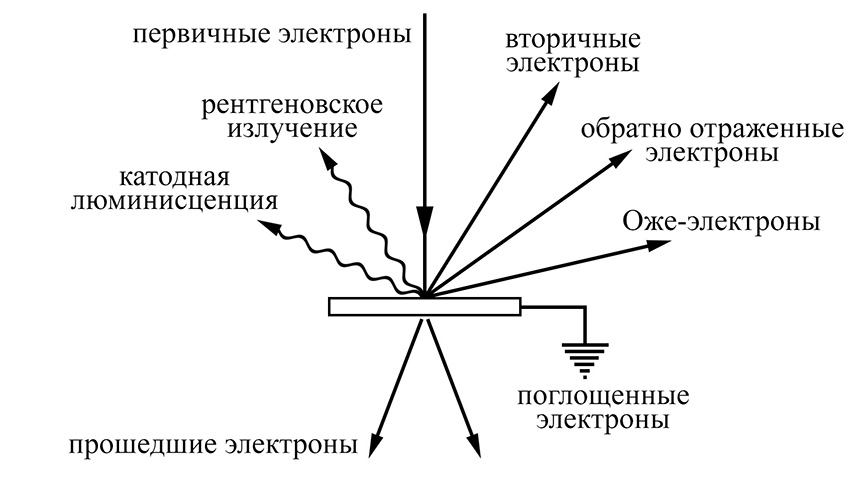
\includegraphics[width=0.95\textwidth]{experiment/REM_1_small}
	\caption{Схема образования вторичных сигналов при взаимодействии электронного пучка с веществом мишени.}
	\label{fig:REM_1}
\end{figure}

Растровый электронный микроскоп является вакуумным прибором, так как при нормальном атмосферном давлении электронный пучок сильно рассеивается и поглощается, что делает невозможным его фокусировку. Давление в рабочей камере микроскопа должно составлять порядка 10$^\text{-5}$ торр или ниже. Схема основных элементов растрового электронного микроскопа приведена на рисунке~\ref{fig:REM_2}. Электронный пучок от источника электронов фокусируется специальной конденсорной системой и проходит через систему управляющих электродов или электромагнитов, которые перемещают пучок по поверхности образца по траектории, образующей растр.

\begin{figure}[t]
	\centering
	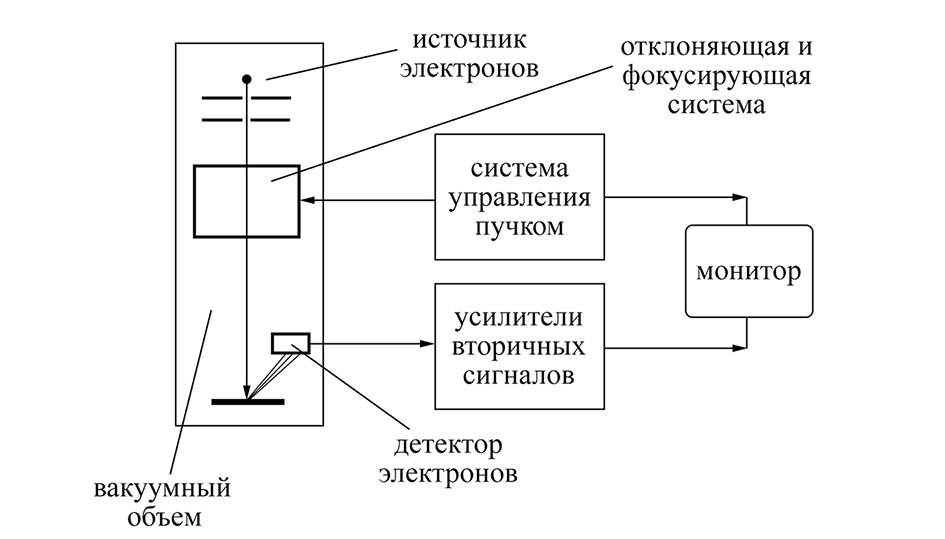
\includegraphics[width=0.95\textwidth]{experiment/REM_2_200}
	\caption{Упрощенная схема, иллюстрирующая работу РЭМ.}
	\label{fig:REM_2}
\end{figure}

Разрешение РЭМ определяется размером области в образце, возбуждаемой электронным пучком, а интенсивность вторичных сигналов --  величиной тока пучка. Таким образом, электронно-оптическая система, формирующая пучок, должна обеспечивать получение максимально возможного тока при минимально возможных поперечных размерах пучка. Электронно-оптическая система включает в себя источник электронов (вольфрамовый катод, катод из гексаборида лантана (LaB$_\text{6}$) или автоэмиссионный катод), модулятор (цилиндра Венельта) и анод (рисунок~\ref{fig:REM_3}). Модулятор обычно имеет отрицательный потенциал в несколько сотен вольт относительно катода, что позволяет сформировать электронный пучок с диаметром $d_0$ и расходимостью $\alpha_0$. Характерные значения $d_0$ и $\alpha_0$ для электронно-оптических систем, используемых в рентгеновских микроанализаторах и растровых электронных микроскопах, составляют 25--100 мкм и 3--10\:$\cdot$\,10$^\text{-3}$ рад соответственно.

\begin{figure}
	\centering
	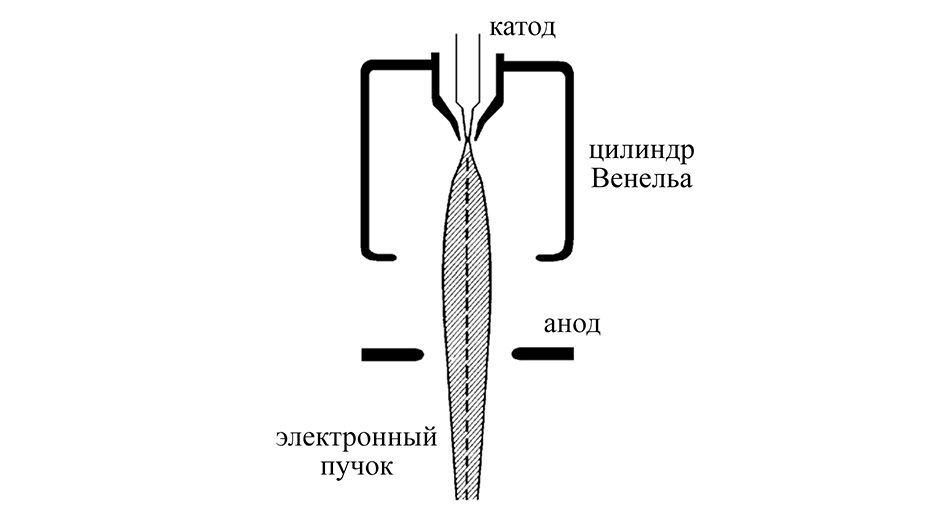
\includegraphics[width=0.95\textwidth]{experiment/REM_3_200}
	\caption{Схема устройства электронно-оптической системы растрового электронного микроскопа.}
	\label{fig:REM_3}
\end{figure}

\paragraph{Сцинтилляционный детектор} \mbox{} \\
\indent В настоящее время наиболее широкое распространение в РЭМ для регистрации вторичных электронов получили сцинтилляционные детекторы. Вторичные электроны попадают на сцинтиллятор, преобразующий энергию электрона в световой импульс, который улавливается фотокатодом, преобразуется в фототок и затем усиливается фотоэлектронным умножителем. Между сцинтиллятором и фотоэлектронным умножителем помещается световод, позволяющий вывести фотоумножитель, крайне чувствительный к внешним электрическим и магнитным полям, за пределы вакуумной камеры РЭМ. Так как большинство используемых сцинтилляторов генерируют свет под действием электронов с энергией более 10 кэВ, на внешнюю поверхность сцинтиллятора наносится тонкий полупрозрачный металлический слой, и на него подается положительное напряжение (порядка 10 кВ) для сбора и ускорения низкоэнергетической части спектра вторичных электронов. Для того, чтобы исключить влияние созданного электрического поля на первичные электроны, сцинтиллятор помещается внутрь цилиндра Фарадея. 

\paragraph{Полупроводниковый детектор} \mbox{} \\
\indent Вторичные электроны, попавшие в материал полупроводника вблизи \textit{p-n}-перехода, обеспечивают образование в нем электронно-дырочных пар, что приводит к появлению тока через \textit{p-n}-переход. Этот ток пропорционален количеству электронов, поглощенных полупроводником. Для получения достаточной величины сигнала ток в дальнейшем усиливается специальными малошумящими усилителями. Электроны должны иметь энергию, достаточную для образования электронно-дырочных пар, поэтому полупроводниковый детектор (ППД) обычно используется для регистрации высокоэнергетической части вторичных электронов.

\paragraph{Детектор излучения катодолюминесценции} \mbox{} \\
\indent Количество света, испускаемого мишенью под воздействием электронного пучка, обычно мало, поэтому для увеличения эффективности регистрации испускаемого света используют специальные эллиптические зеркала. В один из фокусов зеркала помещают мишень, а в другой -- световод-приемник, уводящий свет за пределы вакуумной камеры микроскопа. Далее свет регистрируется фотоэлектронным умножителем, либо спектрометром, позволяющим исследовать распределение испущенного образцом света по длинам волн.

\paragraph{Детекторы рентгеновского излучения} \mbox{} \\
\indent Для регистрации рентгеновского излучения обычно используются два типа систем. Во-первых, применяются кристалл-дифракционные спектрометры с изогнутыми для увеличения светосилы кристаллами-анализаторами. Приемником рентгеновского излучения обычно служит сцинтилляционный детектор. В качестве кристалла-сцинтиллятора обычно используются монокристаллы NaI(Tl). Во-вторых, также применяются энергодисперсионные системы, например, кремний-литиевые детекторы. Энергодисперсионные детекторы имеют существенно более низкое энергетическое разрешение (100--150 эВ) по сравнению с кристалл-дифракционными спектрометрами (менее 10 эВ), однако они получили широкое распространение благодаря возможности регистрации всего спектра вторичных электронов без каких-либо перемещений образца и детектора, а также возможности быстрой обработки спектра на ЭВМ.


\subsection*{Атомно-силовая микроскопия}

В основе принципа работы атомно-силового микроскопа (АСМ) лежит силовое взаимодействие между сторонним телом и поверхностью вещества, для регистрации которого используются специальные датчики, представляющие собой упругую консоль (кантилевер) с острым зондом на конце (рисунок~\ref{fig:AFM_1_2} а)). Сила, действующая на зонд со стороны поверхности, приводит к изгибу кантилевера, и за счет регистрации величины изгиба в разных точках сканируемой поверхности можно определить профиль поверхности.

Качественно работу АСМ можно пояснить на примере сил Ван-дер-Ваальса. Энергия ван-дер-ваальсова взаимодействия двух атомов, находящихся на расстоянии $r$ друг от друга, может быть аппроксимирована потенциалом Леннарда-Джонса (рисунок ~\ref{fig:AFM_1_2} б)):
\begin{equation}
	U_\mathrm{LJ}(r) = U_0\left\{-2\left(\frac{r_0}{r}\right)^6+\left(\frac{r_0}{r}\right)^{12}\right\}.
\end{equation}
Первое слагаемое в скобках описывает дальнодействующее притяжение, обусловленное, диполь-дипольным взаимодействием атомов, второе -- отталкивание атомов на малых расстояниях. Параметр $r_0$ -- равновесное расстояние между атомами, $U_0$ -- значение энергии в положении равновесия. 

Полная энергия системы зонд-образец задается формулой
\begin{equation}
	W_\mathrm{PS}=\iint_{\mathrm{V}_\mathrm{P} \mathrm{V}_\mathrm{S}} U_\mathrm{LJ}\left(r-r^{\prime}\right) n_\mathrm{P}\left(r^{\prime}\right) n_\mathrm{S}(r) d V d V^{\prime}
\end{equation}
где $n_\mathrm{P}(r)$ и $n_\mathrm{S}(r^\prime)$ -- плотности атомов в материале зонда и образца, соответственно. Соответственно, сила, действующая на зонд со стороны поверхности, может быть вычислена следующим образом:
\begin{equation}
	\vec{F}_\mathrm{PS} = -\operatorname{grad}\left(W_\mathrm{PS}\right).
\end{equation}
Такое взаимодействие зонда с образцом имеет сложный характер, однако основные черты взаимодействия, характерного для двух атомов, сохраняются -- зонд АСМ испытывает притяжение со стороны образца на больших расстояниях от его поверхности и отталкивание -- на малых.

Получение изображения рельефа поверхности с помощью АСМ связано с регистрацией малых изгибов упругой консоли зондового датчика, для чего широко используются оптические методы (рисунок~\ref{fig:AFM_2}). Оптическая система АСМ юстируется таким образом, чтобы излучение полупроводникового лазера фокусировалось на консоли зондового датчика, а отраженный пучок попадал в центр фоточувствительной области фотоприемника. В качестве позиционно-чувствительных фотоприемников применяются четырехсекционные полупроводниковые фотодиоды.

\begin{figure}[t]
	\centering
	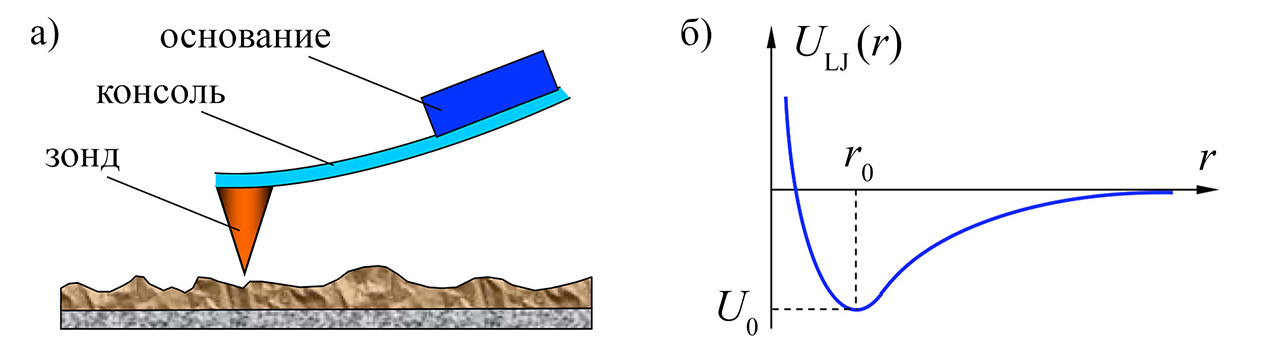
\includegraphics[width=0.9\textwidth]{experiment/AFM_1_2_200}
	\vspace{0.5em}
	\caption{а) Схематическое изображение зондового датчика АСМ, б) качественный вид потенциала Леннарда-Джонса.}
	\label{fig:AFM_1_2}
\end{figure}

Основные регистрируемые оптической системой параметры -- это деформации изгиба консоли под действием $Z$-компонент сил притяжения или отталкивания ($F_\mathrm{Z}$) и деформации кручения консоли под действием латеральных компонент сил ($F_\mathrm{L}$) взаимодействия зонда с поверхностью. Если обозначить исходные значения фототока в секциях фотодиода через $I_{01}$, $I_{02}$, $I_{03}$, $I_{04}$, а через $I_{1}$, $I_{2}$, $I_{3}$, $I_{4}$ -- значения токов после изменения положения консоли, то разностные токи с различных секций фотодиода $\Delta I_i = I_i - I_{0i}$ будут однозначно характеризовать величину и направление изгиба консоли зондового датчика АСМ. Действительно, комбинация разностных токов вида
\begin{equation}
	\Delta I_\mathrm{Z} = \left(\Delta I_1+\Delta I_2\right)-\left(\Delta I_3+\Delta I_4\right)
\end{equation}
пропорциональна изгибу консоли под действием силы, действующей по нормали к поверхности образца, а комбинация вида
\begin{equation}
	\Delta I_\mathrm{L} = \left(\Delta I_1+\Delta I_4\right)-\left(\Delta I_2+\Delta I_3\right)
\end{equation}
характеризует изгиб консоли под действием латеральных сил.

\begin{figure}[t]
	\centering
	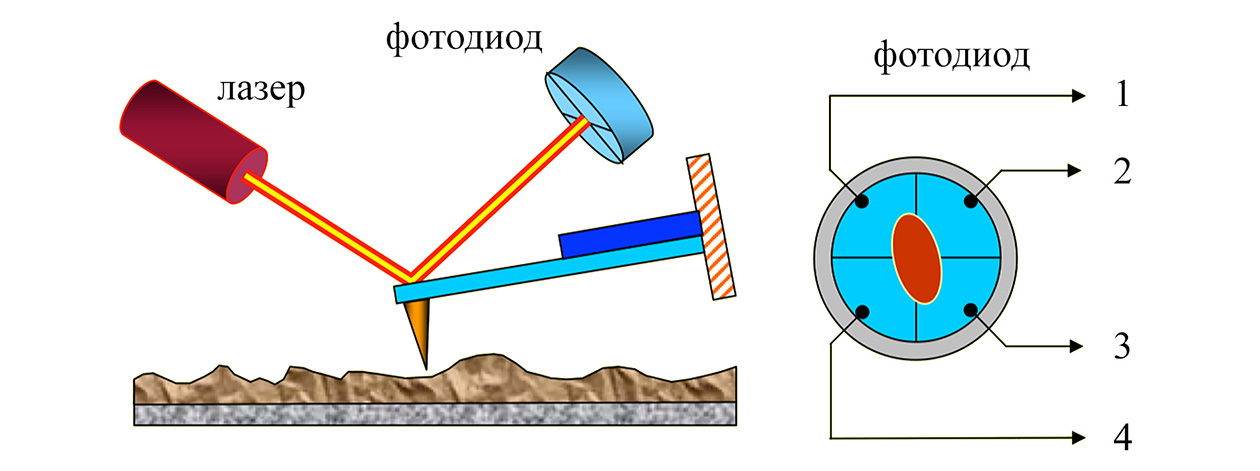
\includegraphics[width=0.9\textwidth]{experiment/AFM_3_200}
	\vspace{0.2em}
	\caption{Схема оптической регистрации изгиба консоли зондового датчика АСМ.}
	\label{fig:AFM_2}
\end{figure}

Величина $\Delta I_\mathrm{Z}$ используется в качестве входного параметра в петле обратной связи атомно-силового микроскопа. Система обратной связи обеспечивает постоянное значение $\Delta I_\mathrm{Z}$ с помощью пьезоэлектрического исполнительного элемента, который поддерживает изгиб консоли $\Delta Z$ равным величине $\Delta Z_0$, задаваемой оператором.

При сканировании образца в режиме $\Delta Z = const$ зонд перемещается вдоль поверхности, при этом напряжение на $Z$-электроде сканера записывается в память компьютера в качестве рельефа поверхности $Z = f(X, Y)$. Пространственное разрешение АСМ определяется радиусом закругления зонда и чувствительностью системы, регистрирующей отклонения консоли. В настоящее время реализованы конструкции АСМ, позволяющие исследовать поверхность образцов с атомарным разрешением.

